\capitulo{5}{Aspectos relevantes del desarrollo del proyecto}

En este apartado se va a comentar, a manera de resumen temporal, el desarrollo del proyecto. Es en este apartado donde se comentarán las opciones y decisiones tomadas, los problemas surgidos y todos los aspectos importantes. Se ha considerado que la mejor forma de organizar este apartado es en seccionaes donde se comenta cada apartado del desarrollo.

\section{Desarrollo FIS-HUBU}\label{desarrolloFH}
FIS-HUBU es una aplicación web que permite realizar vídeo llamadas entre responsables y pacientes con Parkinson para realizar rehabilitaciones de manera \textit{online}, es decir, sin la necesidad de desplazarse hasta la consulta o el hospital. Esta aplicación, que ha sido desarrollada junto con mi compañero José Luis Garrido Labrador, permite por parte del responsable observar y evaluar la evolución del estado de un paciente, esta evolución también es visible para el paciente que puede ver su propio progreso.

La aplicación puede dividirse en distintas partes que serán comentadas a continuación.
\subsection{Vídeo llamadas}
El punto principal de la aplicación, y por ende su principal uso, son las vídeo llamadas entre pacientes y responsables o terapeutas que permitan sustituir la rehabilitaciones presenciales en consulta por rehabilitaciones \textit{online}, permitiendo así que estás se puedan dar más a menudo y puedan ser accesibles para un mayor número de personas, sobre todo para aquellos pacientes que no se pueden desplazar.

Primero se realizó una investigación sobre las principales plataformas de vídeo llamadas. Lo que se estaba buscando de estas plataformas era:
\begin{itemize}
	\item Creación de llamadas de manera sencilla y automática. Si es posible a partir de url.
	\item Vídeo llamada estable sin necesidad de una gran conexión.
	\item Plataforma que permita grabar la cámara de los pacientes.
	\item Plataforma gratuita.
\end{itemize}

Dentro de las plataformas que se investigaron están las más conocidas aplicaciones de este tipo como puede ser \textit{Skype}, pero al final se decidió utilizar \textit{Jitsi} ya que proporciona todas las necesidades anteriormente comentadas, y además permite en un futuro poder crear un servidor propio donde poder modificar parámetros como la calidad de las llamadas.

\subsection{Responsable}
Parte de la aplicación donde los responsables pueden realizar las siguientes tareas:
\begin{itemize}
	\item Iniciar un vídeo llamada con un paciente.
	\item Evaluar la evolución de los pacientes.
	\item Modificar las evaluaciones de los pacientes.
	\item Comprobar la evolución de los pacientes.
\end{itemize}

La interfaz de la aplicación para tipo de usuario es sencilla y clara, como se puede ver en el menú principal, figura~\ref{fig:menuPaciente}, o en el menú de estadísticas, figuras~\ref{fig:menuest} y~\ref{fig:ejemploest}.

\begin{figure}[h]
	\centering
	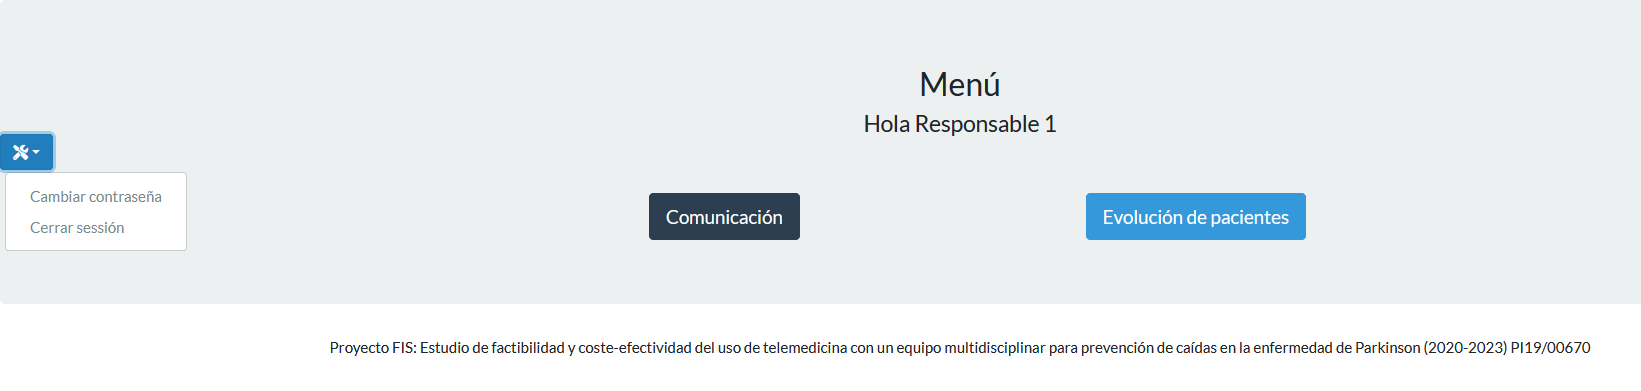
\includegraphics[width=1\textwidth]{menuResponsable}
	\caption{Menú principal de un responsable.}
	\label{fig:menuPaciente}
\end{figure}

\begin{figure}[h]
	\centering
	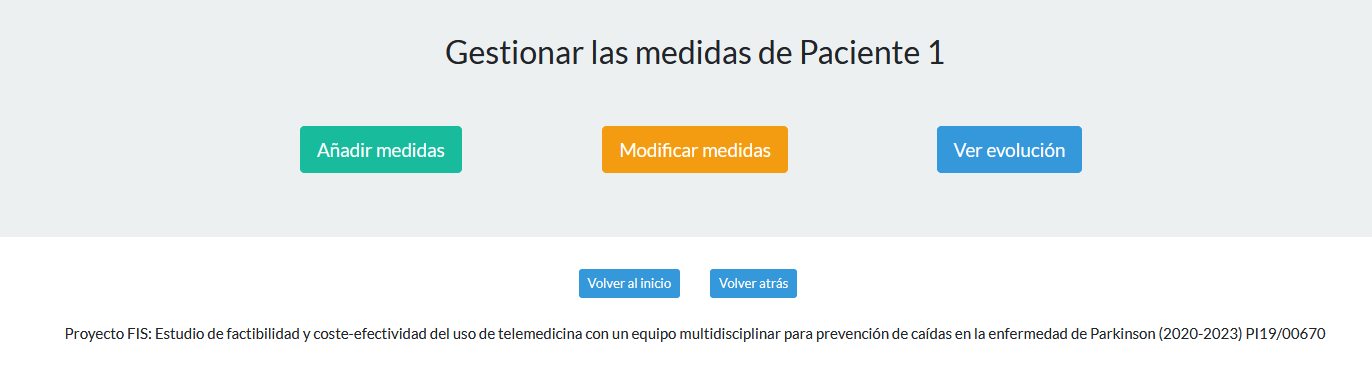
\includegraphics[width=1\textwidth]{menuestad}
	\caption{Menú de estadísticas.}
	\label{fig:menuest}
\end{figure}

\begin{figure}[h]
	\centering
	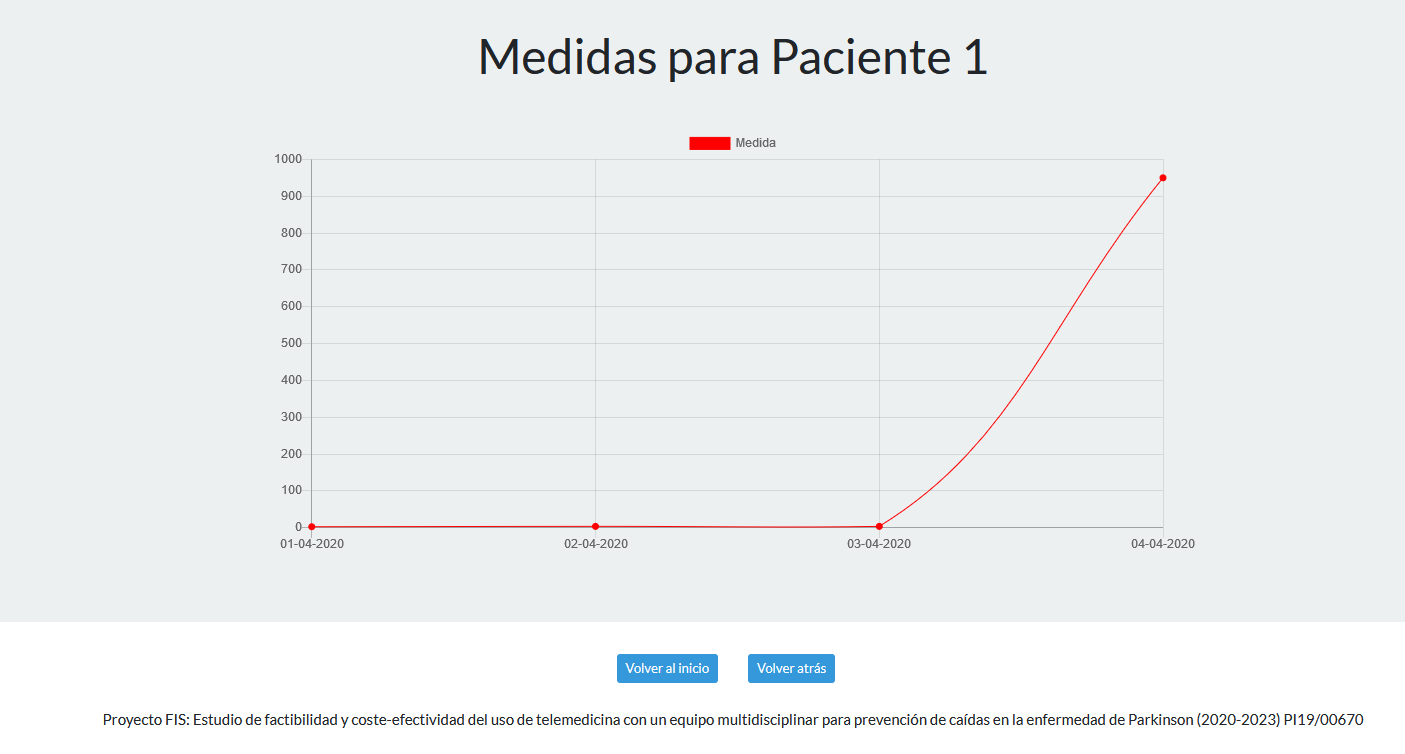
\includegraphics[width=1\textwidth]{ejemploest}
	\caption{Ejemplo de la evolución de un paciente vista por un responsable.}
	\label{fig:ejemploest}
\end{figure}

\subsection{Paciente}
Los pacientes que van a utilizar la aplicación, son pacientes mayores con Parkinson. Esto se ha tenido muy en cuenta tanto en el diseño como en la creación de la parte de la aplicación orientada en los pacientes, se ha intentado que esta parte sea lo más accesible posible, para que todos los pacientes puedan manejarse bien con la aplicación y así poder sacarle el mayor provecho.

Para poder realizar una aplicación lo más accesible posible primero se ha de saber la forma que van a tener los pacientes de interactuar con ésta. En este caso los pacientes van a utilizar un mando de SNES\footnote{SNES: \textit{Super Nintendo Entertainment System}} con botones de colores, es por ello que se ha aprovechado estos colores para poder mostrar en la interfaz de la aplicación que botón han de pulsar para realizar que acción. Además, se ha creado un botón de ayuda que carga una página donde se puede ver la acción que realiza cada botón del mando. Un ejemplo de la interfaz de esta aplicación se puede ver en la figura~\ref{fig:menupaciente}.

\begin{figure}[h]
	\centering
	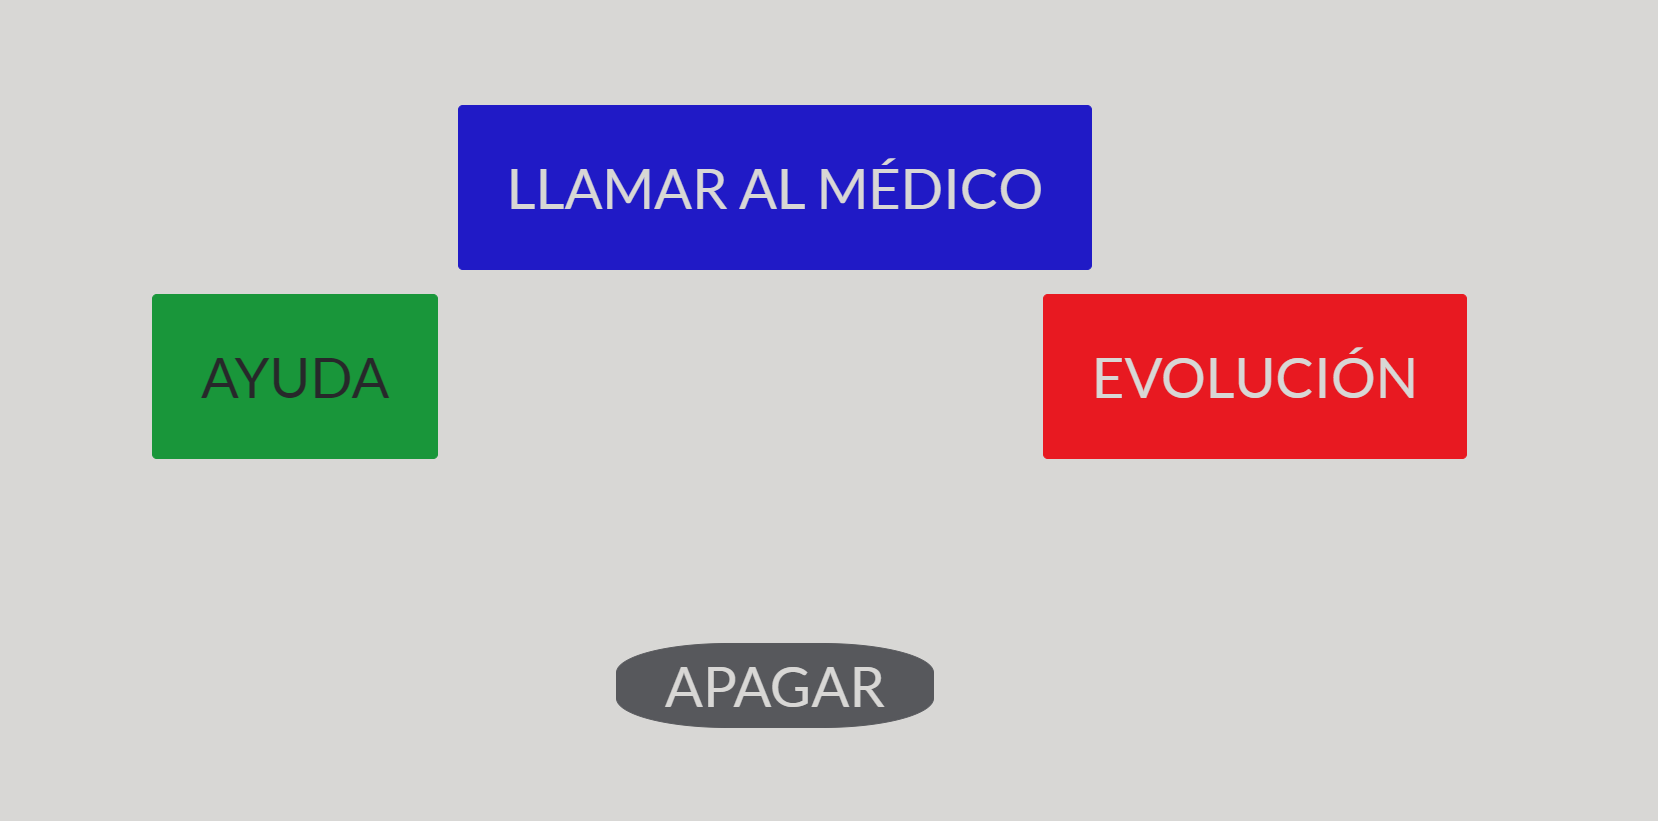
\includegraphics[width=1\textwidth]{menupac}
	\caption{Menú principal de los pacientes.}
	\label{fig:menupaciente}
\end{figure}

\subsection{Dispositivos necesarios}
Para poder utilizar la aplicación se necesitan distintos dispositivos, que dependiendo del tipo de usuario (responsable o paciente) son unos u otros.

Para los responsables lo único que se necesita es un ordenador con conexión a \textit{Internet} y una cámara conectada a éste.

Por otro lado, los pacientes se presupone que no disponen de ningún dispositivo capaz de cargar la aplicación, es por ello que a cada paciente se le proporciona:
\begin{itemize}
	\item MSI
	\item CAMARA
\end{itemize}

\subsection{Conexión}
Como ya se ha comentado, el principal uso de la aplicación es las rehabilitaciones \textit{online} para pacientes, mayoritariamente de tercera edad, que no se pueden desplazar a las consultas. Muchas de estas personas mayores viven en lugares donde no se tiene contratada ninguna línea de \textit{Internet}, es por ello que además del desarrollo de la aplicación se contrató una serie de \textit{routers} 4G para poder proporcionar conexión a los dispositivos necesarios. 

\section{Investigación algoritmos de visión por computador}
Tras haber desarrollado la versión inicial, donde en un futuro se quiere añadir lo resultados de este proyecto, se pasó a realizar la primera investigación sobre los distintos algoritmos de visión por computar capaces de detectar y seguir los movimientos de una persona. 

De estos algoritmos se necesita:
\begin{itemize}
	\item Posibilidad de cargar un modelo existente o crear un modelo capaz de detectar a la persona que sale en la imagen.
	\item Posibilidad de cargar un modelo existente o crear un modelo capaz de detectar la posición de la persona.
	\item Que el procesado de nuevos fotogramas para detectar a la persona y su posición se realicé en poco tiempo.
	\item Que la salida del procesado de los fotogramas pueda servir para una posterior comparación con el ejercicio base.
\end{itemize}

Teniendo todos estos factores en cuenta se estudió qué herramientas se pueden usar para esta fase del trabajo. Se buscó herramientas programadas en \textit{Python} para poder conectarse bien con el resto del proyecto y porque es uno de los lenguajes con los cuales se tiene más soltura, tanto por parte del alumno como por parte de los tutores para resolver dudas y ayudar en los problemas. Las herramientas encontradas fuera:
\begin{itemize}
	\item \textit{TF-Pose-EStimator}.
	\item \textit{PoseNet}.
	\item \textit{Detectron2}.
\end{itemize}

De cada una de estas herramientas se realizó una investigación y experimentación para probar si cumplían las necesidades requeridas. Al finalizar esta etapa, la única herramienta que permitía realizar todas las necesidades era \textit{Detectron2}. Además, permite con un modelo ya creado por los propios desarrolladores realizar las tareas de predicción de elementos y de la posición de la persona.

\section{Investigación de \textit{Detectron2}}
PROBLEMAS CON EL GUARDADO DE VÍDEO Y EXTRACCIÓPN DE LAS CARACTERISTICAS
PONER EL UMBRAL, PONER COMO MEJORA CMABIANDO EL UMBRAL 